%%%%%%%%%%%%%%%%%%%% paper.tex %%%%%%%%%%%%%%%%%%%%%%%%%%%%%%%%%%%
%
% Root file for QMI-CFS manuscript (empirical-study restructure)
%
% Based on Springer SVProc template
%
%%%%%%%%%%%%%%%% Springer %%%%%%%%%%%%%%%%%%%%%%%%%%%%%%%%%%

\documentclass{svproc}

% Required packages
\usepackage{amsmath,amssymb}
\usepackage{graphicx}
\usepackage{booktabs}
\usepackage{multirow}
\usepackage{url}
\usepackage{xcolor}
\usepackage{algorithm}
\usepackage{algpseudocode}
\usepackage{caption}
\usepackage{subcaption}
\usepackage{tikz}
\usetikzlibrary{shapes.geometric, arrows, positioning, fit}

\def\UrlFont{\rmfamily}

% Shortcuts
\newcommand{\QMI}{I_Q}
\newcommand{\MI}{I}
\newcommand{\vn}{S}
\newcommand{\D}{\mathcal{D}}

% Theorem-like environments
\newtheorem{observation}{Observation}
\newtheorem{theorem}{Theorem}
\newtheorem{corollary}{Corollary}

\begin{document}
\mainmatter

\title{Quantum Mutual Information for Causal Feature Selection: An Empirical Study of Feature Recovery and Treatment Effect Estimation}
%
\titlerunning{QMI-CFS for Confounder Selection}
%
\author{Anonymous Author(s)}
%
\authorrunning{Anonymous et al.}
%
\tocauthor{Anonymous Author(s)}
%
\institute{Anonymous Institution,\\
\email{anonymous@institution.edu}}

\maketitle

\begin{abstract}
We investigate whether Quantum Mutual Information (QMI), a quantum-information-theoretic dependency measure, provides a useful perspective on causal feature selection. Through six synthetic datasets and the IHDP benchmark, we evaluate QMI-based confounder recovery alongside classical information-theoretic and tree-based selectors, and we examine how well feature-selection accuracy predicts downstream treatment-effect estimation quality. Results show that QMI is competitive with classical methods while avoiding the bandwidth or neighbor-count choices of k-NN mutual information and the kernel hyperparameter choices of RKHS dependence measures. More importantly, confounder recovery and causal estimation quality are only weakly correlated: across the six synthetic DGPs, F1 score explains only about 4\% of the variance in ATE error. The IHDP benchmark exemplifies this divergence, with QMI-CFS achieving the lowest ATE error despite only moderate F1. These findings suggest that future evaluation of causal feature-selection methods should jointly consider feature recovery and downstream causal performance, and that quantum-inspired dependency measures are best understood as structured, parameter-free alternatives to classical kernel-based scores rather than sources of quantum advantage.
\keywords{Quantum Mutual Information, Causal Inference, Feature Selection, Treatment Effect Estimation, Quantum-Inspired Methods}
\end{abstract}

\section{Introduction}
\label{sec:intro}

Estimating treatment effects from observational data requires adjusting for confounding variables that influence both treatment assignment and outcome. The validity of causal estimates depends critically on the correct identification of these confounders - a feature selection problem with profound downstream consequences \cite{pearl2009causality,imbens2015causal}.

Classical feature selection methods for causal inference include mutual information (MI) \cite{fleuret2004fast}, conditional mutual information (CMI) \cite{tsamardinos2003algorithms}, LASSO \cite{tibshirani1996regression}, Boruta \cite{kursa2010boruta}, and random forest importance \cite{breiman2001random}. These methods have complementary strengths: MI and CMI are principled but rely on density estimation, LASSO is computationally efficient but assumes linearity, and tree-based wrappers capture interactions but lack strong identification guarantees and can be unstable in small samples.

Quantum information theory offers a structurally different way to measure dependencies. Quantum Mutual Information (QMI), defined through von Neumann entropy of density matrices, operates on quantum states obtained by embedding classical data into a Hilbert space \cite{havlivcek2019supervised,schuld2021supervised}. The resulting criterion is deterministic and parameter-free at estimation time: once the encoding is fixed, no bandwidth or neighbor-count parameter must be chosen, in contrast to k-NN MI \cite{kraskov2004estimating} and kernel-based dependence measures such as HSIC \cite{gretton2005measuring,gretton2007kernel}. Importantly, \textbf{we do not claim that QMI detects dependencies ``invisible'' to classical methods, nor do we claim any quantum advantage}. Rather, this paper treats QMI as a quantum-inspired dependency measure that provides a structured, parameter-free lens for studying causal feature selection.

\textbf{What this paper is not.} This is \textit{not} a paper claiming a universally superior confounder selector, a quantum speedup, or a quantum advantage. All computations are classical simulations of small quantum systems. The paper is an empirical study: we use QMI as a representative quantum-information-theoretic dependency measure to understand the behavior of dependency-based confounder selection.

\textbf{Research questions.} This paper pursues three questions:
\begin{enumerate}
    \item[RQ1] Can Quantum Mutual Information identify confounders competitively with classical information-theoretic methods?
    \item[RQ2] Does improved confounder recovery necessarily lead to improved treatment-effect estimation?
    \item[RQ3] What limitations do dependency-based confounder selection methods face under interaction confounding?
\end{enumerate}

\textbf{Contributions.} Our principal contributions are:
\begin{enumerate}
    \item \textbf{Framework:} We present QMI-CFS, a quantum-inspired information-theoretic framework for ranking candidate confounders by QMI computed from density matrices, relate QMI to classical mutual information via dephasing (Observation~\ref{obs:qmi_bound}), prove a finite-sample concentration bound (Theorem~\ref{thm:qmi_concentration}) and ranking-consistency corollary (Corollary~\ref{cor:ranking}), and analyze the default weight choice $(\alpha,\beta,\gamma)=(0.4,0.4,0.2)$ and its limitations.
    \item \textbf{Empirical comparison:} We report a systematic comparison of QMI-CFS against classical information-theoretic and tree-based selectors across six synthetic datasets and IHDP, evaluating both feature recovery and downstream ATE estimation.
    \item \textbf{Divergence finding:} We provide evidence that confounder-recovery metrics and causal-estimation metrics are only weakly correlated. Across the six synthetic DGPs, F1 score explains approximately 4\% of the variance in ATE error; excluding the interaction-confounded IC dataset, it explains about 2\%.
    \item \textbf{Limitation analysis:} We show that dependency-based selectors, including QMI-CFS, struggle under interaction-driven confounding, and that pairwise QMI augmentation and nonlinear AIPW provide only small, inconsistent gains.
\end{enumerate}

\section{Related Work}
\label{sec:related}

\subsection{Feature Selection for Causal Inference}

Information-theoretic feature selection ranks features by mutual information $I(X;Y)$ \cite{koller1996toward}. For causal inference, CMI $I(X;Y \mid T)$ conditions on treatment to identify confounders \cite{yu2020causality}. Both MI and CMI rely on density estimation (histograms or k-NN), which suffers from high variance when $n < 5d$ \cite{kraskov2004estimating}. LASSO provides sparse selection but assumes linearity; nonlinear confounders are systematically missed \cite{belloni2014inference}. Tree-based wrappers such as Boruta capture interactions but lack theoretical guarantees for causal identification and can be computationally expensive for small samples \cite{kursa2010boruta}.

Recent work has explicitly connected mutual information to causal effect estimation. Kiriakidou and Diou \cite{kiriakidou2024mutual} use MI-based neighbor selection for treatment effect estimation, while transfer-entropy methods have been widely applied to causal discovery in time series \cite{schreiber2000measuring}. Gao and Aragam \cite{gao2021efficient} provide finite-sample guarantees for local Markov boundary search. These works show that classical information-theoretic criteria remain strong baselines when carefully estimated.

\subsection{Small-Sample Treatment Effect Estimation}

Curth and van der Schaar \cite{curth2021inductive} analyze inductive biases for heterogeneous treatment effect estimation in small samples, emphasizing that no single representation is universally optimal. Curth et al. \cite{curth2021really} provide a critical assessment of the IHDP benchmark, showing that performance differences are sensitive to implementation details and that ``all features'' can be surprisingly competitive. Their critique motivates our honest reporting of baseline performance.

\subsection{Quantum Machine Learning and Kernel Methods}

Quantum feature maps embed classical data into Hilbert space via parameterized quantum circuits \cite{havlivcek2019supervised}. Schuld \cite{schuld2021supervised} showed that supervised quantum models can be understood as kernel methods in a quantum feature Hilbert space. From this perspective, QMI-CFS is related to classical kernel-based dependency measures: angle encoding followed by density-matrix construction defines a particular feature map, and QMI measures entropy in that mapped space. However, QMI differs from kernel-based dependence measures such as HSIC \cite{gretton2005measuring,gretton2007kernel,gretton2012kernel} in important ways. HSIC estimates the squared norm of the cross-covariance operator in a reproducing kernel Hilbert space and requires choosing a kernel bandwidth. QMI instead estimates the von Neumann entropy of density matrices built from the same feature map; it is parameter-free at estimation time and bounded by the dimension of the density matrix. A classical kernel method with a similarly designed feature map and carefully tuned bandwidth could capture analogous dependencies; the potential value of QMI-CFS lies in the specific regularization induced by the trace-one density-matrix geometry and the absence of bandwidth hyperparameters.

Quantum feature selection has been explored via QUBO formulations \cite{mucke2023feature} and quantum annealing \cite{mummaneni2024miqubo}, but these approaches use classical MI as the objective and employ quantum hardware only for combinatorial optimization. Flores-Garrig\'{o}s et al. \cite{flores2026quantum} use higher-order binary optimization with classical MI coefficients on trapped-ion hardware. To our knowledge, no prior work uses von-Neumann-entropy-based QMI itself as the selection criterion for causal inference.

We distinguish our use of ``QMI'' (Quantum Mutual Information) from ``QMIFS'' \cite{vergara2017qmifs}, which stands for Quadratic Mutual Information Feature Selection and is a purely classical method based on quadratic R\'{e}nyi entropy.

\subsection{Quantum Information Theory}

Von Neumann entropy $\vn(\rho) = -\operatorname{Tr}(\rho \log \rho)$ generalizes Shannon entropy to quantum states \cite{nielsen2010quantum}. Quantum Mutual Information $\QMI(A;B) = \vn(\rho_A) + \vn(\rho_B) - \vn(\rho_{AB})$ measures correlations in bipartite quantum systems \cite{vedral2002role}. We apply these quantities to classically simulated quantum states constructed from observational data.

\section{Preliminaries}
\label{sec:prelim}

\paragraph{Notation.} Let $D = \{(\mathbf{x}_i, t_i, y_i)\}_{i=1}^n$ denote observational data with covariates $\mathbf{x} \in \mathbb{R}^d$, binary treatment $t \in \{0,1\}$, and continuous outcome $y \in \mathbb{R}$. The Average Treatment Effect (ATE) is $\tau = \mathbb{E}[Y(1) - Y(0)]$. We assume the backdoor criterion holds: all confounders are observed and there exists a set $S \subseteq \{1,\dots,d\}$ such that treatment assignment is ignorable conditional on $\mathbf{X}_S$ \cite{pearl2009causality,imbens2015causal}.

\paragraph{Quantum States and Density Matrices.} A quantum state is represented by a density matrix $\rho$, a Hermitian positive semi-definite matrix with $\operatorname{Tr}(\rho) = 1$. For a pure state $|\psi\rangle$, $\rho = |\psi\rangle\langle\psi|$.

\paragraph{Von Neumann Entropy.} For density matrix $\rho$ with eigenvalues $\{\lambda_k\}$:
\begin{equation}
    \vn(\rho) = -\sum_k \lambda_k \log_2 \lambda_k
\end{equation}

\paragraph{Quantum Mutual Information.} For a bipartite system with joint density matrix $\rho_{AB}$ and marginals $\rho_A = \operatorname{Tr}_B(\rho_{AB})$, $\rho_B = \operatorname{Tr}_A(\rho_{AB})$:
\begin{equation}
    \label{eq:qmi}
    \QMI(A;B) = \vn(\rho_A) + \vn(\rho_B) - \vn(\rho_{AB})
\end{equation}

\paragraph{Conditional QMI.} Extending to three subsystems:
\begin{equation}
    \label{eq:conditional_qmi}
    \QMI(A;B \mid C) = \vn(\rho_{AC}) + \vn(\rho_{BC}) - \vn(\rho_C) - \vn(\rho_{ABC})
\end{equation}
This expression follows from the chain rule for von Neumann entropy and is non-negative by strong subadditivity.

\paragraph{Interpreting conditional QMI for confounder selection.} For the product-state construction used here, conditioning on $Y$ removes the shared variation between $X_j$ and $Y$ before measuring the residual dependency between $X_j$ and $T$. A feature with high $\QMI(X_j; T)$ but low $\QMI(X_j; T \mid Y)$ is predictive of treatment but not outcome, and is therefore likely an instrument rather than a confounder. We emphasize that conditional QMI is used as a ranking term that helps distinguish confounders from instruments; it is not intended as an exact conditional independence test, because the angle-encoded density matrix only approximates the underlying classical conditional distribution.

\section{The QMI-CFS Framework}
\label{sec:method}

QMI-CFS comprises seven stages: observed data, preprocessing, quantum encoding, QMI computation, confounder selection, treatment effect estimation, and outputs. Figure~\ref{fig:pipeline} illustrates the pipeline.

\begin{figure}[htbp]
    \centering
    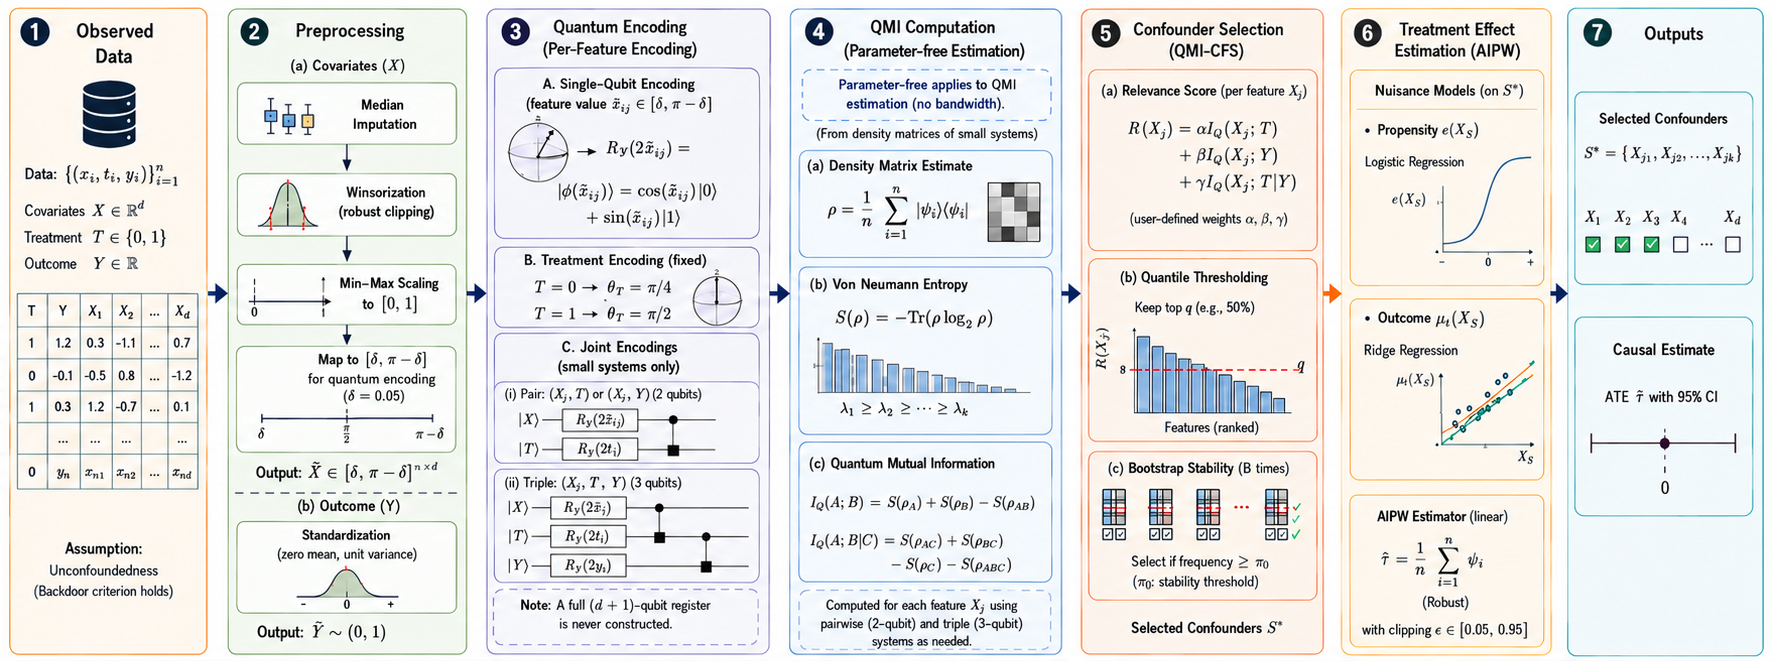
\includegraphics[width=\textwidth]{figures/Pipeline.png}
    \caption{QMI-CFS pipeline. Data are preprocessed, angle-encoded into quantum states, and summarized by density matrices of small (single-, pair-, and triple-qubit) systems; QMI is computed without bandwidth selection. Features are scored by the composite relevance function $\mathcal{R}(X_j)$ and selected via quantile thresholding and bootstrap stability. The final ATE is estimated with a linear doubly-robust AIPW estimator. All quantum operations are simulated classically; a full $(d+1)$-qubit register is never constructed.}
    \label{fig:pipeline}
\end{figure}

\subsection{Quantum Encoding}
\label{subsec:encoding}

We employ angle encoding with $R_Y$ rotation gates. Each preprocessed feature value $\tilde{x}_{ij}$ is mapped from $[0,1]$ to $[\delta, \pi-\delta]$ via
\begin{equation}
    \tilde{x}_{ij} = \delta + (\pi - 2\delta)\,\frac{x_{ij}^{\text{norm}} - \min_k x_{kj}^{\text{norm}}}{\max_k x_{kj}^{\text{norm}} - \min_k x_{kj}^{\text{norm}}},
\end{equation}
where $x^{\text{norm}}$ is a winsorized and median-imputed version of the raw feature, and $\delta = 0.05$. The single-qubit state is
\begin{equation}
    |\phi(x_i^{(j)})\rangle = R_Y(2\tilde{x}_{ij})|0\rangle = \cos(\tilde{x}_{ij})|0\rangle + \sin(\tilde{x}_{ij})|1\rangle.
\end{equation}
The binary treatment is encoded with fixed angles, $T=0 \to \theta_T=\pi/4$ and $T=1 \to \theta_T=\pi/2$, so that $|\phi(t_i)\rangle$ is a pure state on the Bloch sphere.

For joint systems, we apply linear CZ entanglement between adjacent qubits:
\begin{equation}
    U_{\phi}(\mathbf{x}_i) = \left(\bigotimes_{j=1}^d R_Y(2\tilde{x}_{ij})\right) \cdot \left(\prod_{j=1}^{d-1} \text{CZ}_{j,j+1}\right).
\end{equation}
Importantly, QMI-CFS never constructs a full $(d+1)$-qubit register. Each QMI term is computed from small density matrices: single-qubit marginals for $\QMI(X_j;T)$ and $\QMI(X_j;Y)$, two-qubit joint matrices for the pair terms, and three-qubit joint matrices for the conditional term $\QMI(X_j;T \mid Y)$.

\subsection{Density Matrix Construction}
\label{subsec:density}

For single-qubit systems, the density matrix is constructed analytically from data:
\begin{equation}
    \rho_{X_j} = \frac{1}{n}\sum_{i=1}^n |\phi(x_i^{(j)})\rangle\langle\phi(x_i^{(j)})| = \begin{pmatrix} a_j & c_j \\ c_j & 1-a_j \end{pmatrix}
\end{equation}
where $a_j = \frac{1}{2}(1 + \frac{1}{n}\sum_i \cos 2\tilde{x}_{ij})$ and $c_j = \frac{1}{2n}\sum_i \sin 2\tilde{x}_{ij}$.

For two-qubit joint systems (feature + treatment):
\begin{equation}
    \rho_{X_j,T} = \frac{1}{n}\sum_{i=1}^n |\psi_i\rangle\langle\psi_i|, \quad |\psi_i\rangle = |\phi(x_i^{(j)})\rangle \otimes |\phi(t_i)\rangle
\end{equation}
with CZ entanglement introducing phase flips on the $|11\rangle$ component.

\subsection{QMI Computation}
\label{subsec:qmi_compute}

Given density matrices, we compute QMI via eigenvalue decomposition:
\begin{enumerate}
    \item Compute eigenvalues $\{\lambda_k\}$ of each density matrix
    \item Clip eigenvalues to $[10^{-12}, 1]$ for numerical stability
    \item Evaluate von Neumann entropy and apply Eq.~(\ref{eq:qmi})
\end{enumerate}

For each feature $X_j$, we compute three QMI terms:
\begin{itemize}
    \item $\QMI(X_j; T)$: propensity relevance
    \item $\QMI(X_j; Y)$: prognostic relevance
    \item $\QMI(X_j; T \mid Y)$: conditional relevance (distinguishes confounders from instruments)
\end{itemize}

\subsection{Feature Selection}
\label{subsec:selection}

\begin{algorithm}[htbp]
\caption{QMI-CFS Feature Selection}
\label{alg:selection}
\begin{algorithmic}[1]
\Require Preprocessed dataset $\tilde{D}$, weights $(\alpha, \beta, \gamma)$, quantile $q$, bootstrap $B$, stability threshold $\pi_0$
\Ensure Selected feature subset $S^*$
\For{each feature $j = 1, \dots, d$}
    \State Compute $\QMI(X_j; T)$, $\QMI(X_j; Y)$, $\QMI(X_j; T \mid Y)$
    \State $\mathcal{R}(X_j) = \alpha \cdot \QMI(X_j; T) + \beta \cdot \QMI(X_j; Y) + \gamma \cdot \QMI(X_j; T \mid Y)$
\EndFor
\State $S_0 = \{j : \mathcal{R}(X_j) \geq \text{Quantile}_q(\{\mathcal{R}(X_k)\})\}$
\For{$b = 1, \dots, B$}
    \State Resample $\tilde{D}^{(b)}$ with replacement
    \State Recompute $\mathcal{R}^{(b)}(X_j)$ for $j \in S_0$
    \State $S^{(b)} = \{j \in S_0 : \mathcal{R}^{(b)}(X_j) \geq \text{Quantile}_q(\{\mathcal{R}^{(b)}(X_k)\})\}$
\EndFor
\State $S^* = \{j \in S_0 : \frac{1}{B}\sum_b \mathbb{1}\{j \in S^{(b)}\} \geq \pi_0\}$
\State \Return $S^*$
\end{algorithmic}
\end{algorithm}

The composite relevance score balances three criteria:
\begin{equation}
    \label{eq:relevance}
    \mathcal{R}(X_j) = \alpha \cdot \QMI(X_j; T) + \beta \cdot \QMI(X_j; Y) + \gamma \cdot \QMI(X_j; T \mid Y)
\end{equation}

We employ a two-stage selection procedure (Algorithm~\ref{alg:selection}). First, a quantile-based initial screen keeps the upper half of features ($q=0.5$). Second, bootstrap stability screening resamples the data $B$ times (default $B=100$; focused experiments use $B=20$ for computational feasibility) and retains only those initial candidates selected in at least a fraction $\pi_0=0.6$ of replications. Unlike fixed-$k$ selection, the final subset size is data-driven.

The default weights $(\alpha, \beta, \gamma) = (0.4, 0.4, 0.2)$ give equal emphasis to propensity and prognostic relevance while using the conditional term as a tie-breaker that penalizes instruments. This choice mirrors common practice in confounder selection, where balancing treatment and outcome predictiveness is prioritized \cite{vansteelandt2012model}. The conditional term receives a smaller weight because it is used primarily to break ties between features that are similarly relevant to treatment and outcome, not to dominate the score.

\paragraph{Why these weights?} The weight choice reflects a qualitative prior: a good confounder must be predictive of both treatment and outcome, so $\alpha$ and $\beta$ receive the largest shares. Setting $\alpha=\beta$ avoids privileging either propensity or prognostic information a priori. The conditional term $\QMI(X_j; T \mid Y)$ helps distinguish instruments (features predictive of treatment but not outcome) from true confounders, but it is noisier than the marginal terms in small samples; hence $\gamma=0.2$ is kept small. Table~\ref{tab:ablation} confirms that the default is a stable compromise: the Conservative configuration $(1/3,1/3,1/3)$ and the Precision configuration $(0.2,0.6,0.2)$ trade recall for precision in a dataset-dependent way, but no single alternative dominates across DGPs.

\paragraph{How could the weights be improved?} The current weights are fixed hyperparameters. A principled improvement would be to select them by cross-validating the downstream ATE error or feature-recovery F1 on a held-out subset of the data. Because the composite score is differentiable only indirectly through the selected set, one could use a small grid search over $(\alpha,\beta,\gamma)$ on a validation DGP and choose the configuration that minimizes ATE error. Alternatively, one could learn dataset-specific weights from a meta-training set of DGPs with known causal structure. Both directions are left for future work; the fixed default is intentionally simple and avoids introducing additional tuning into the empirical comparison.

\paragraph{Pairwise interaction augmentation (exploratory).} When confounders enter through multiplicative interactions, a feature may have only weak marginal relevance. We optionally augment the per-feature score with a pairwise interaction term computed once on the full data. For each feature $X_j$, we compute the pairwise QMI matrix $\mathbf{M}_{jk} = \QMI(X_j; X_k)$, identify the top-$k^*$ features with highest $M_{jk}$, and set $\mathcal{P}(X_j) = \max_{k^*} M_{jk^*}$. The final relevance score is $(1-\lambda) \mathcal{R}(X_j) + \lambda \mathcal{P}(X_j)$, with $\lambda=0.2$. As we report in Section~\ref{sec:ablation}, this augmentation yields only small and inconsistent gains; it is best viewed as an exploratory sensitivity analysis rather than a core component of QMI-CFS.

\subsection{Treatment Effect Estimation}
\label{subsec:ate}

Using selected features $S^*$, we estimate the ATE via Augmented Inverse Probability Weighting (AIPW):
\begin{equation}
    \label{eq:aipw}
    \hat{\tau}_{\text{AIPW}} = \frac{1}{n}\sum_{i=1}^n \left[\hat{\mu}_1(\mathbf{x}_i) - \hat{\mu}_0(\mathbf{x}_i) + \frac{T_i}{\hat{e}(\mathbf{x}_i)}\bigl(Y_i - \hat{\mu}_1(\mathbf{x}_i)\bigr) - \frac{1-T_i}{1-\hat{e}(\mathbf{x}_i)}\bigl(Y_i - \hat{\mu}_0(\mathbf{x}_i)\bigr)\right]
\end{equation}
where $\hat{e}(\mathbf{x}_i)$ is the estimated propensity score and $\hat{\mu}_t(\mathbf{x}_i)$ are estimated potential-outcome means conditional on the selected covariates. By default propensity scores are estimated via logistic regression with clipping at $[0.05, 0.95]$, and outcomes are modeled with ridge regression. For settings with nonlinear confounding, the AIPW estimator can be configured with arbitrary sklearn-compatible propensity and outcome models. Our experiments with random-forest nuisance models are reported as an exploratory sensitivity analysis in Section~\ref{sec:interacting}; they do not represent a fully tuned nonlinear causal estimation pipeline.

\section{Theoretical Analysis}
\label{sec:theory}

\begin{observation}[QMI upper-bounds classical MI]
\label{obs:qmi_bound}
Let $\rho_{AB}$ be a bipartite quantum state constructed from classical data via angle encoding, and let $P(A,B)$ be the corresponding classical joint distribution obtained by measuring $\rho_{AB}$ in the computational basis. Let $\D(\rho_{AB})$ denote the fully dephased (diagonal) state. Then:
\begin{equation}
    \QMI(A;B) \geq \MI(A;B)
\end{equation}
with equality whenever $\QMI(A;B) = \QMI(\D(\rho_{AB}))$, i.e., when coherence terms do not contribute to the mutual information.
\end{observation}

\textit{Proof sketch.} The dephasing channel $\D$ is unital and leaves the diagonal distribution invariant, so $\MI(A;B) = \QMI(\D(\rho_{AB}))$. QMI is monotone under the completely positive trace-preserving map $\D$ \cite{nielsen2010quantum}, hence $\QMI(A;B) \geq \QMI(\D(\rho_{AB})) = \MI(A;B)$. \qed

This observation places QMI in context: it measures dependency in a feature space induced by angle encoding, and it is guaranteed to capture at least the classical mutual information. It is a structural property, not a finite-sample guarantee or a claim of superiority over classical methods.

\begin{theorem}[Concentration of finite-sample QMI]
\label{thm:qmi_concentration}
Let $\rho$ be a density matrix constructed from $n$ i.i.d. samples via angle encoding with a fixed preprocessing mapping to $[\delta, \pi-\delta]$, and let $\rho^*$ be the population density matrix. Let $\widehat S_n(\rho)$ denote the von Neumann entropy computed with eigenvalues clipped to $[\epsilon, 1-\epsilon]$. Then there exists a constant $C$ depending only on $\delta$, $\epsilon$, and the dimension of $\rho$ such that, for any $\alpha \in (0,1)$,
\begin{equation}
    \mathbb{P}\bigl(|\widehat S_n(\rho) - S(\rho^*)| \ge C/\sqrt{n} \cdot \sqrt{\log(1/\alpha)}\bigr) \le \alpha.
\end{equation}
Consequently, for any two features $X_j$, $X_k$ and treatment/outcome pair $(T,Y)$, the estimated QMI satisfies
\begin{equation}
    |\widehat{\QMI}_n(X_j; T) - \QMI(X_j; T)| \le C/\sqrt{n} \cdot \sqrt{\log(1/\alpha)}
\end{equation}
with probability at least $1-\alpha$, and similarly for $\QMI(X_j; Y)$ and $\QMI(X_j; T \mid Y)$.
\end{theorem}

\textit{Proof sketch.} Each entry of the empirical density matrix is an average of i.i.d. bounded random variables (sines and cosines of the encoded features). By Hoeffding's inequality, every entry concentrates around its population expectation at rate $O(1/\sqrt{n})$. For Hermitian matrices, Weyl's inequality bounds eigenvalue perturbations by the operator-norm perturbation of the matrix, which is controlled by the entrywise deviations. With eigenvalue clipping at $\epsilon$, the map from eigenvalues to von Neumann entropy is Lipschitz, so the entropy concentrates at the same rate. QMI is a finite sum of such entropies, hence the result. \qed

\begin{corollary}[Ranking consistency]
\label{cor:ranking}
Let $X_j$ and $X_k$ be two features with population QMI scores satisfying $\QMI(X_j; T) > \QMI(X_k; T) + \gamma$ for some $\gamma > 0$. Then there exists $n_0 = O(\log(1/\alpha)/\gamma^2)$ such that for all $n \ge n_0$,
\begin{equation}
    \mathbb{P}\bigl(\widehat{\QMI}_n(X_j; T) > \widehat{\QMI}_n(X_k; T)\bigr) \ge 1 - \alpha.
\end{equation}
\end{corollary}

\textit{Proof sketch.} Apply Theorem~\ref{thm:qmi_concentration} with error smaller than $\gamma/3$. Then $\widehat{\QMI}_n(X_j; T) > \QMI(X_j; T) - \gamma/3 > \QMI(X_k; T) + 2\gamma/3 > \widehat{\QMI}_n(X_k; T) + \gamma/3$. \qed

Theorem~\ref{thm:qmi_concentration} and Corollary~\ref{cor:ranking} strengthen the theoretical footing of QMI-CFS: the estimated dependency scores are consistent, and the ranking of features by QMI stabilizes as sample size grows. The $O(1/\sqrt{n})$ rate is the same order as standard kernel density estimators, but it is obtained here without any bandwidth selection. The fixed-preprocessing assumption is standard for such concentration statements; in practice the empirical min/max scaling converges to fixed population bounds, so the same asymptotic conclusions hold.

\section{Relationship to Kernel Dependency Measures}
\label{sec:kernel}

QMI-CFS is closely related to classical kernel-based dependency measures. Angle encoding maps a classical feature $x$ to a quantum state $|\phi(x)\rangle$, which can be viewed as a nonlinear feature map $\phi: \mathbb{R} \to \mathcal{H}$ into a two-dimensional Hilbert space. The density matrix $\rho = \frac{1}{n}\sum_i |\phi(x_i)\rangle\langle\phi(x_i)|$ is then the empirical covariance operator of these mapped features, normalized to unit trace. From this perspective, QMI operates on the same kind of feature-space geometry as kernel methods.

\paragraph{Similarities.} Kernel dependence measures such as HSIC \cite{gretton2005measuring,gretton2007kernel} also map data into a (possibly infinite-dimensional) feature space and quantify dependence through cross-covariance in that space. For appropriately chosen kernels, HSIC and related kernel-MI estimators can capture the same nonlinear dependencies as QMI.

\paragraph{Differences.} Three differences are worth highlighting. First, QMI uses von Neumann entropy of density matrices rather than an RKHS norm or covariance operator, so it does not require choosing a kernel bandwidth at estimation time. Second, the trace-one normalization of the density matrix provides a built-in geometric regularization. Third, QMI-CFS combines propensity, prognostic, and conditional QMI terms into a single composite score, whereas HSIC measures undirected dependence.

\paragraph{Interpretation.} QMI-CFS should therefore be understood as a quantum-inspired dependency measure operating in a feature space induced by angle encoding. It is not claimed to access dependencies unavailable to classical methods, but it offers a parameter-free, geometrically regularized alternative to bandwidth-dependent kernel scores. A direct empirical comparison with HSIC-based selectors is left for future work.

\section{Experimental Design}
\label{sec:experiments}

\subsection{Datasets}

Table~\ref{tab:datasets} summarizes the six synthetic datasets and the IHDP benchmark. The synthetic DGPs are designed to span linear, nonlinear, high-dimensional, correlated, weakly confounded, and interacting-confounder settings. All synthetic datasets use $n=500$ to study the moderate-sample regime; small-sample behavior is examined separately in Section~\ref{sec:small_sample} by subsampling a fixed DGP at $n \in \{100, 250, 500, 1000\}$.

\input{tables/table1_datasets.txt}

\subsection{Baselines}

We compare against classical information-theoretic, regularization, tree, and All-Features baselines:
\begin{itemize}
    \item \textbf{MI:} Classical mutual information via k-NN estimation
    \item \textbf{CMI:} Conditional mutual information $I(X; Y \mid T)$
    \item \textbf{LASSO:} Post-double selection (logistic for $T$, Lasso for $Y$)
    \item \textbf{Boruta:} Random Forest wrapper with shadow features
    \item \textbf{All-Features:} No selection (baseline for ATE estimation)
\end{itemize}

Additional methods such as HSIC-based selectors \cite{gretton2005measuring,gretton2007kernel}, BART \cite{hill2011bayesian}, Causal Forest \cite{wager2018estimation}, and DragonNet \cite{shi2019adapting} would strengthen the comparison; their inclusion is left for future work.

\subsection{Metrics and Statistical Testing}

\textbf{Feature Selection:} Precision, Recall, and F1-score for confounder identification.

\textbf{Treatment Effect Estimation:} $\text{ATE Error} = |\hat{\tau} - \tau_{\text{true}}|$.

\textbf{Statistical Testing:} Paired t-tests (Experiment 1) and Wilcoxon signed-rank tests (Experiment 2, 3, IHDP) with Holm-Bonferroni correction ($\alpha = 0.05$).

\section{Results}
\label{sec:results}

\subsection{Feature Recovery}

Table~\ref{tab:f1} reports confounder-recovery F1 scores across the six synthetic datasets. QMI-CFS outperforms MI on five of six datasets and LASSO on five of six, but it is not universally dominant: tree-based wrappers (Boruta) achieve the highest F1 on several DGPs, CMI is best on the interaction-confounded setting, and LASSO is best on the weak-confounding setting. These results answer RQ1 affirmatively - QMI is competitive with classical information-theoretic selectors - while confirming that no single method dominates feature recovery.

\input{tables/table2_f1.txt}

\subsection{Treatment Effect Estimation}

Table~\ref{tab:ate} shows ATE estimation errors. LASSO and All-Features are often competitive, especially on linear or low-dimensional settings, because the downstream AIPW model is linear/Ridge. QMI-CFS reduces ATE error relative to MI on five of six datasets (all except NLC), suggesting that the QMI-based selection is generally more robust than k-NN MI for the downstream linear AIPW estimator, though not uniformly.

\input{tables/table3_ate.txt}

\begin{figure}[htbp]
    \centering
    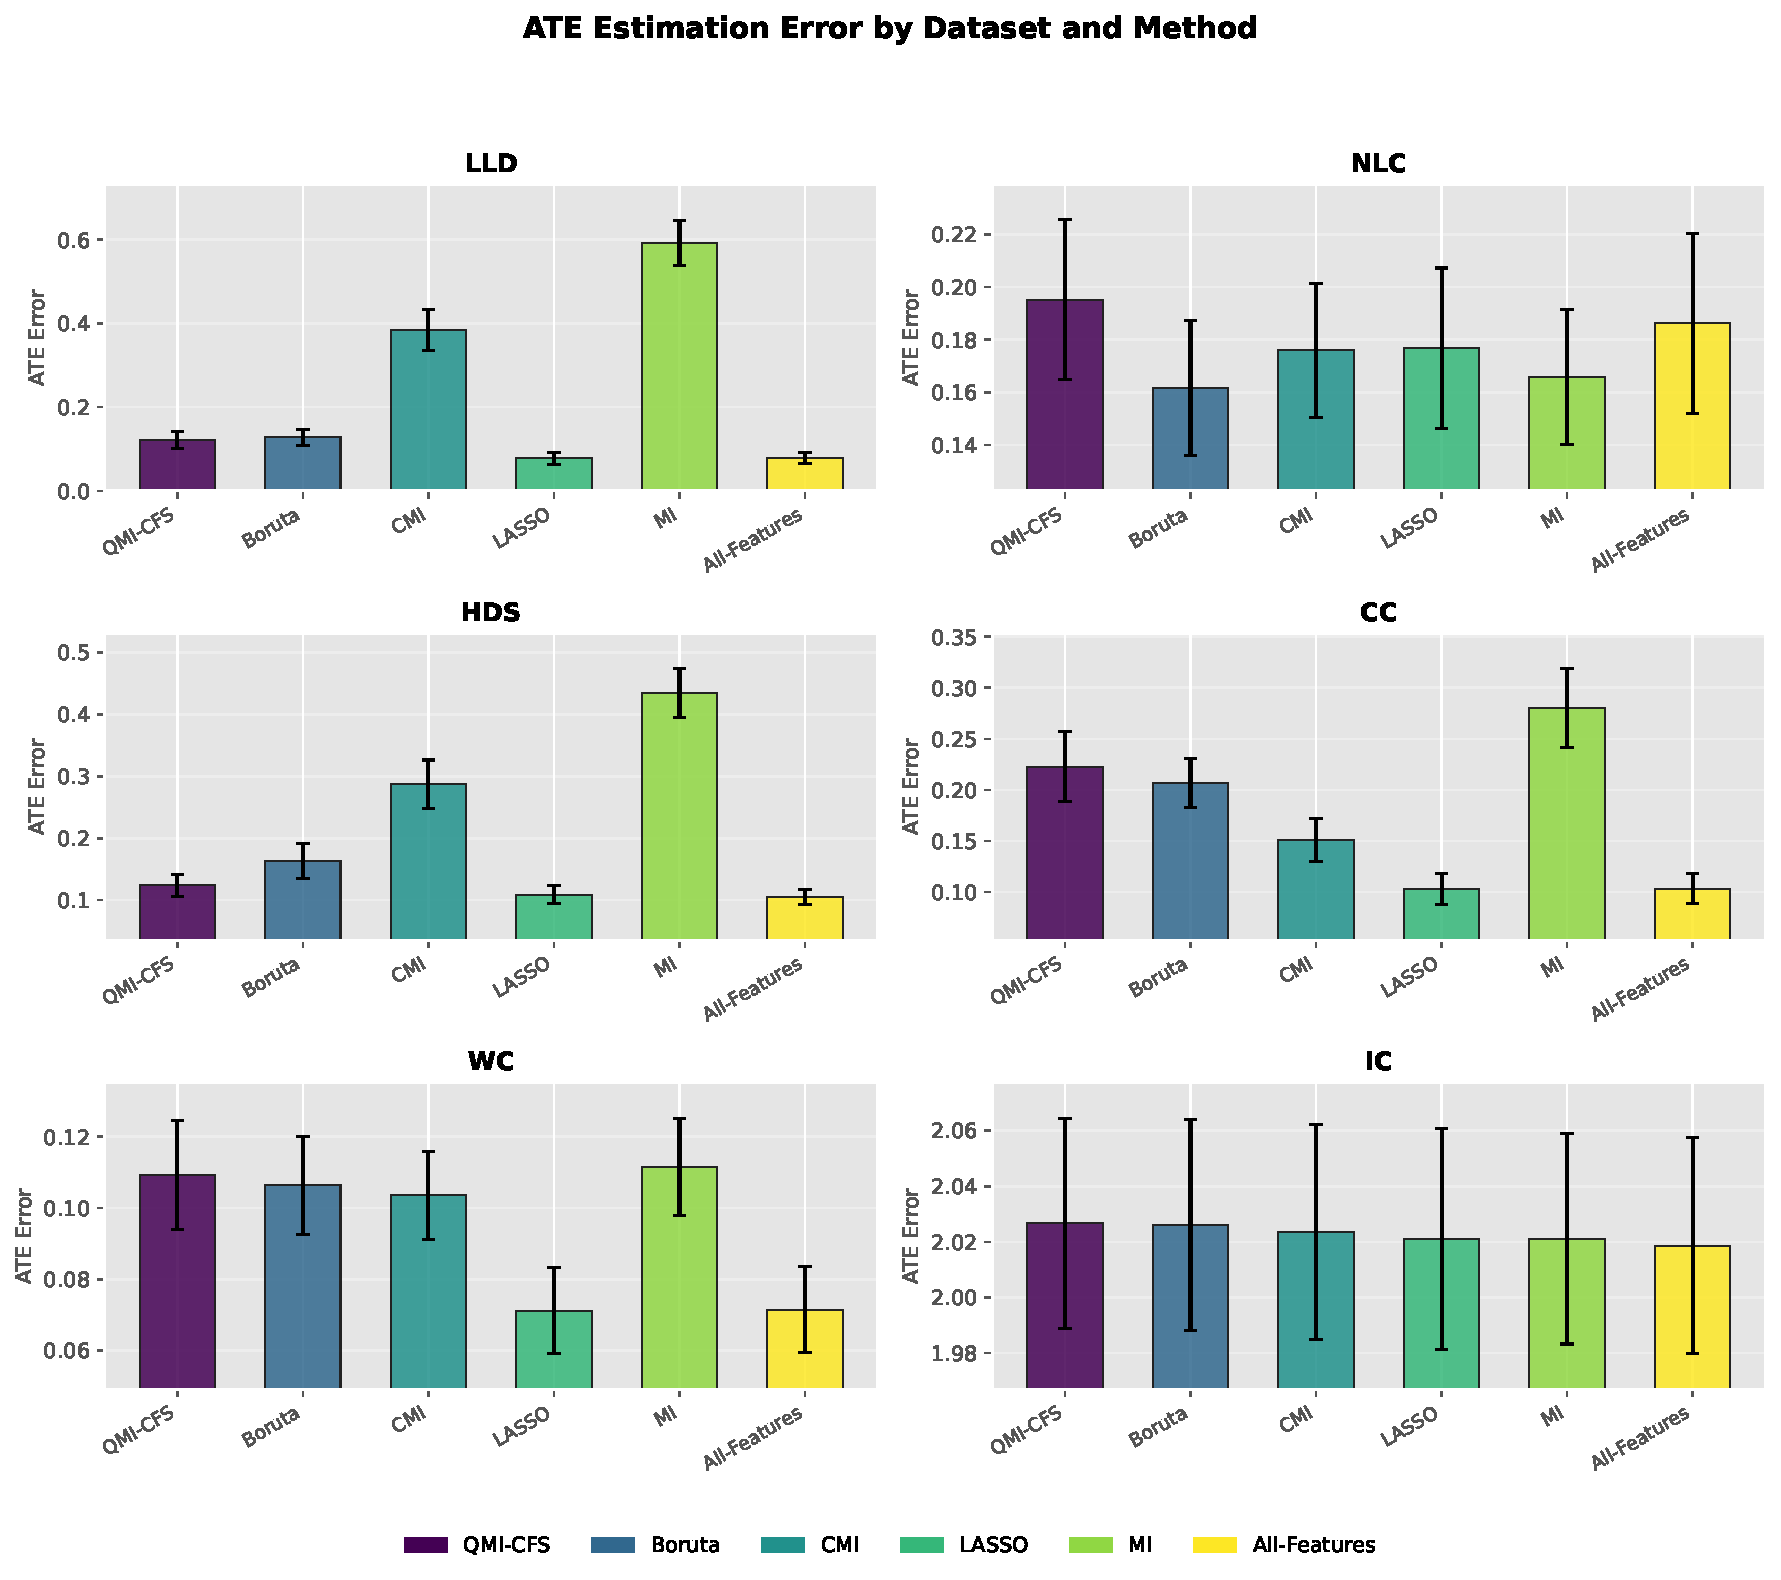
\includegraphics[width=\textwidth]{figures/v3_experiment2_ate.pdf}
    \caption{ATE estimation error by dataset and method (3$\times$2 grid). Each panel has an independent y-axis so method differences are visible even when datasets have very different error scales. Error bars show standard error.}
    \label{fig:ate}
\end{figure}

The IC dataset reveals a striking pattern: every method has ATE error $\approx 2.0$, i.e., roughly $100\%$ relative error. Because both propensity and outcome depend on multiplicative interactions $X_j X_k$, a linear AIPW estimator cannot recover the true treatment effect even when the interacting features are selected.

\subsection{Feature Recovery vs. Causal Estimation Quality}

The central empirical question of this paper is whether better confounder recovery translates into better treatment-effect estimation. Figure~\ref{fig:f1_ate_by_dataset} plots mean F1 score against mean ATE error separately for each synthetic DGP. The overall relationship across the six synthetic DGPs is weak: Pearson correlation $r=-0.201$ ($p=0.287$, $R^2=0.040$), and Spearman's $\rho=0.115$. Thus, F1 score explains only about $4\%$ of the variance in ATE error. Excluding the interaction-confounded IC dataset, the correlation is even closer to zero ($r=0.153$, $R^2=0.023$). Within individual datasets the correlations vary in sign and are not statistically significant, confirming that confounder-recovery metrics do not reliably predict causal-estimation performance.

\begin{figure}[htbp]
    \centering
    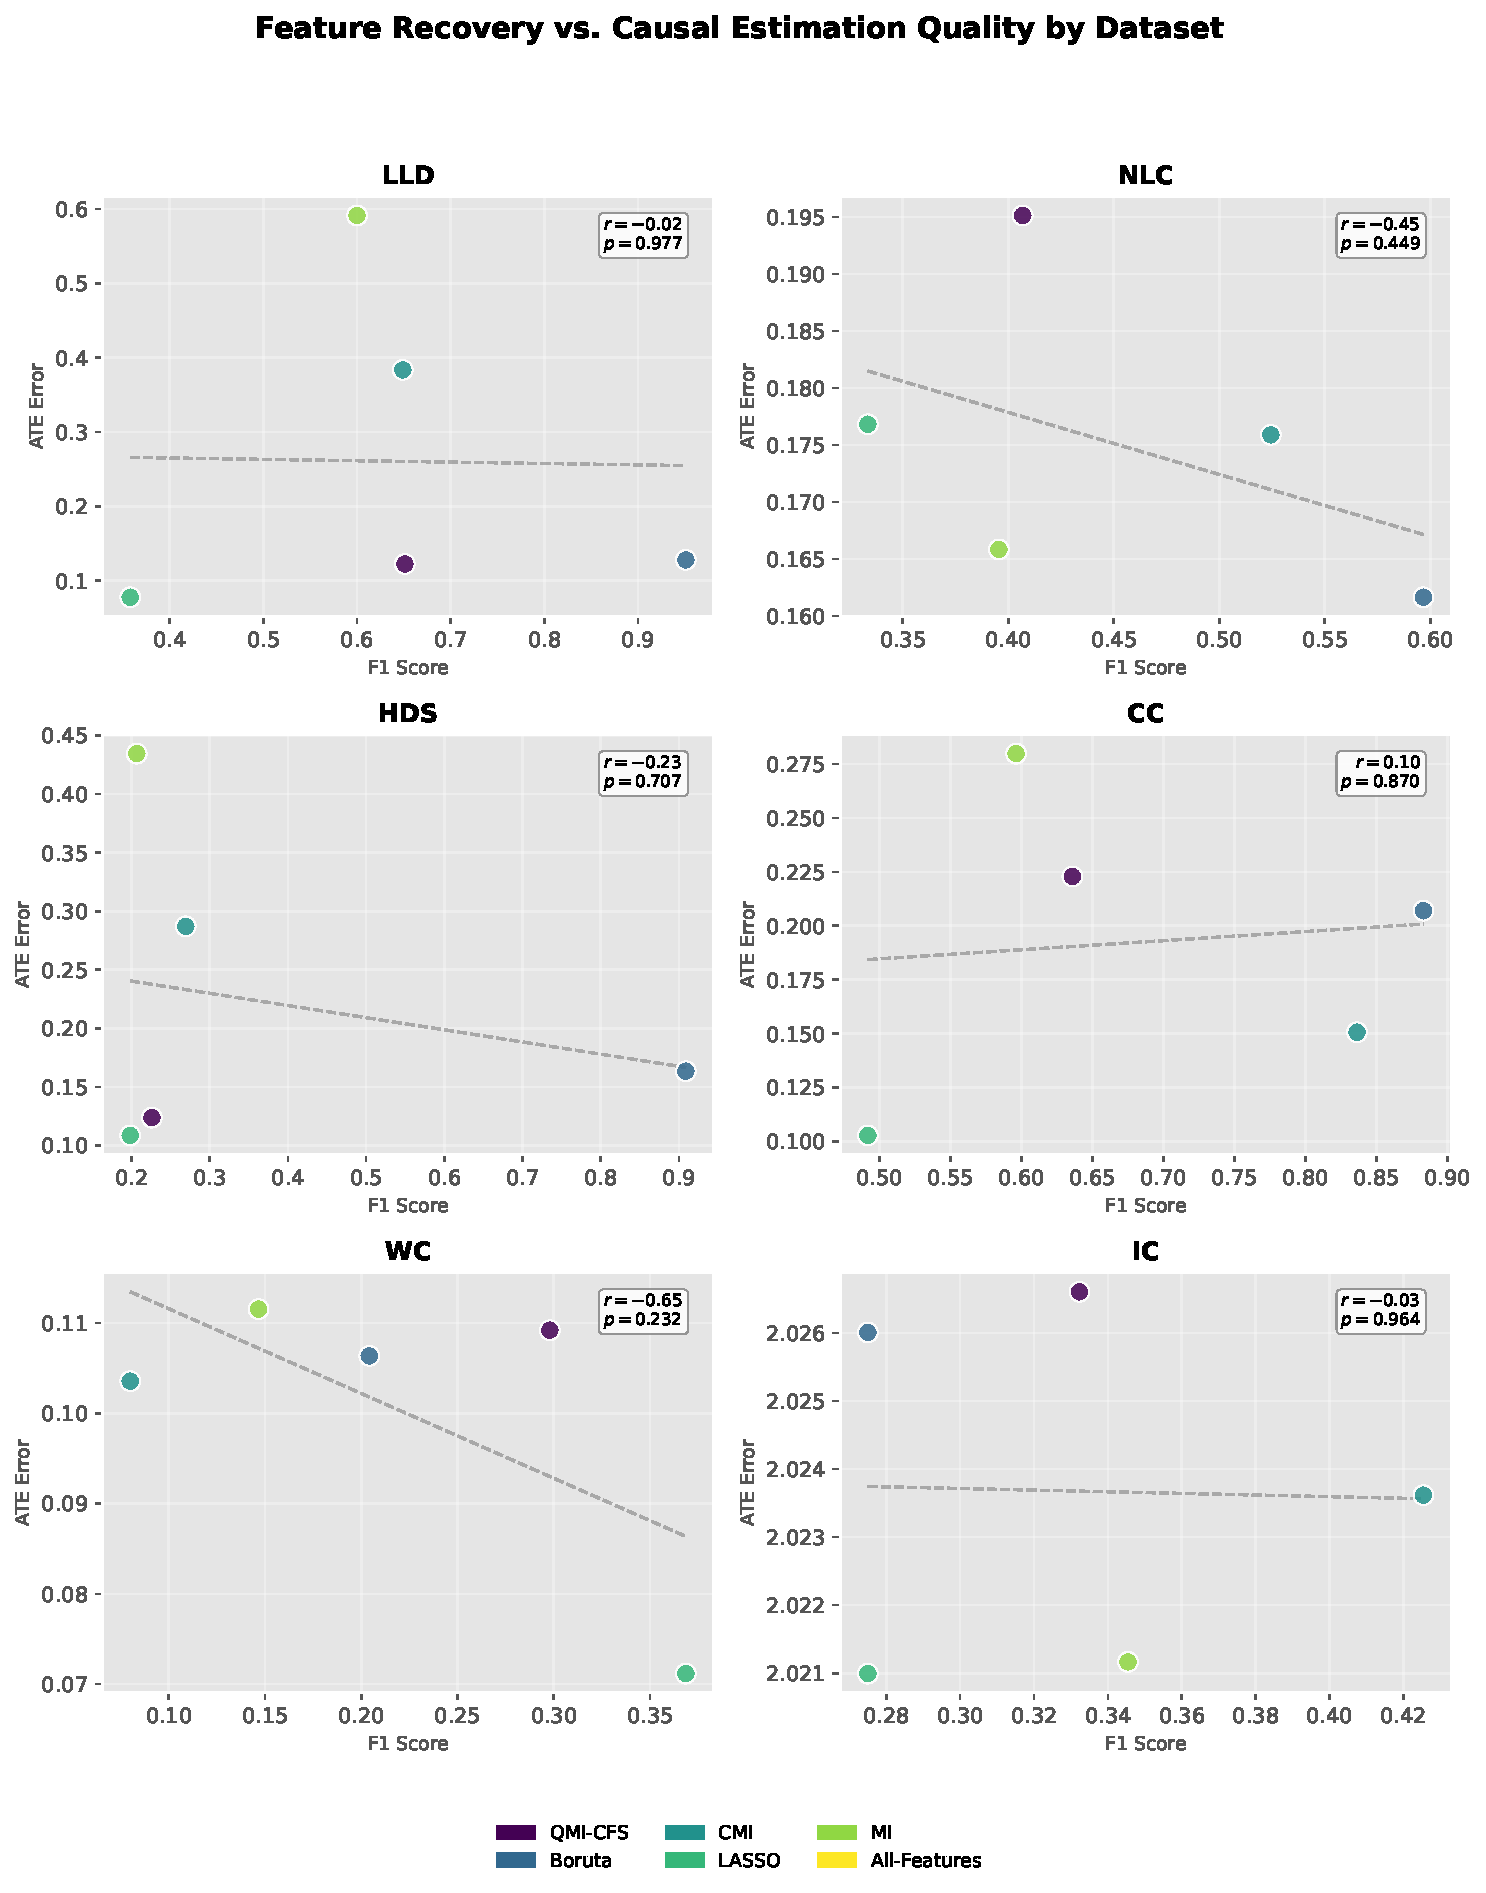
\includegraphics[width=\textwidth]{figures/v5_f1_vs_ate_by_dataset.pdf}
    \caption{Feature recovery (F1) versus treatment-effect estimation error (ATE) for each of the six synthetic DGPs. Each panel reports the Pearson correlation and $p$-value for that DGP; correlations vary in sign and magnitude, indicating that confounder-recovery metrics do not reliably predict causal-estimation performance.}
    \label{fig:f1_ate_by_dataset}
\end{figure}

Table~\ref{tab:ihdp} reports the IHDP Setting A results, and Figure~\ref{fig:ihdp} visualizes the recovery-estimation divergence.

\input{tables/table5_ihdp.txt}

\begin{figure}[htbp]
    \centering
    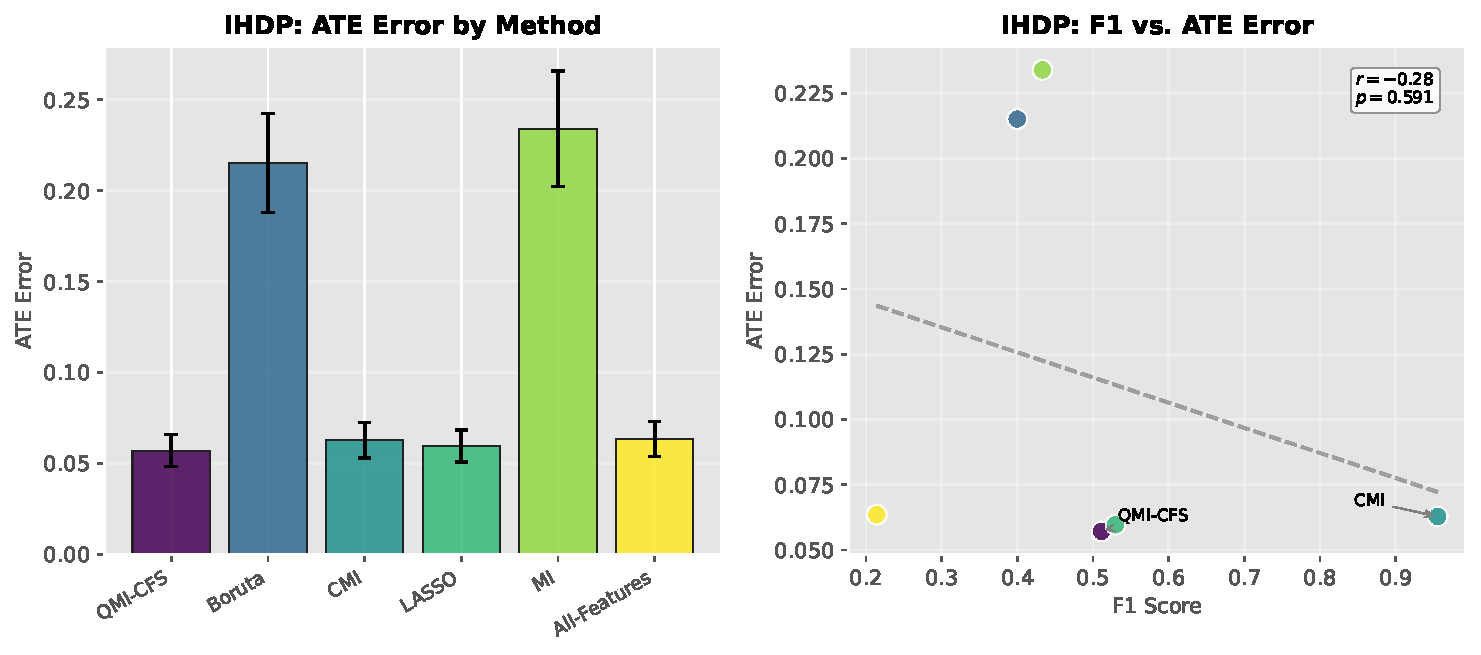
\includegraphics[width=\textwidth]{figures/v5_ihdp_combined.pdf}
    \caption{IHDP Setting A: ATE error by method (left) and the recovery-estimation trade-off with a linear regression line (right). QMI-CFS achieves the lowest ATE error despite only moderate F1, illustrating the divergence between confounder recovery and causal estimation quality.}
    \label{fig:ihdp}
\end{figure}

The IHDP benchmark is the clearest example of this divergence (Figure~\ref{fig:ihdp}). CMI achieves the highest F1 ($0.956$), while QMI-CFS has a more modest F1 of $0.511$. \textit{Despite this, QMI-CFS achieves the lowest ATE error} ($0.057$), slightly better than LASSO ($0.060$), CMI ($0.063$), and All-Features ($0.063$). MI performs poorly on both metrics (F1 $0.433$, ATE error $0.234$). This single dataset demonstrates that a feature set with lower recovery accuracy can nonetheless yield more accurate causal estimates, presumably because it is better calibrated for the downstream nuisance models.

\subsection{Small-Sample Behavior}
\label{sec:small_sample}

Table~\ref{tab:small_sample} and Figure~\ref{fig:small_sample} show F1 score and ATE error as functions of sample size on the LLD DGP. QMI-CFS improves consistently with $n$: F1 rises from $0.450$ at $n=100$ to $0.787$ at $n=1000$, and ATE error falls from $0.681$ to $0.072$. By $n=500$-$1000$, QMI-CFS is competitive with or better than MI, CMI, and LASSO. Boruta dominates feature recovery across all sample sizes, while LASSO and All-Features maintain low ATE error because the DGP is approximately linear.

\input{tables/table4_small_sample.txt}

\begin{figure}[htbp]
    \centering
    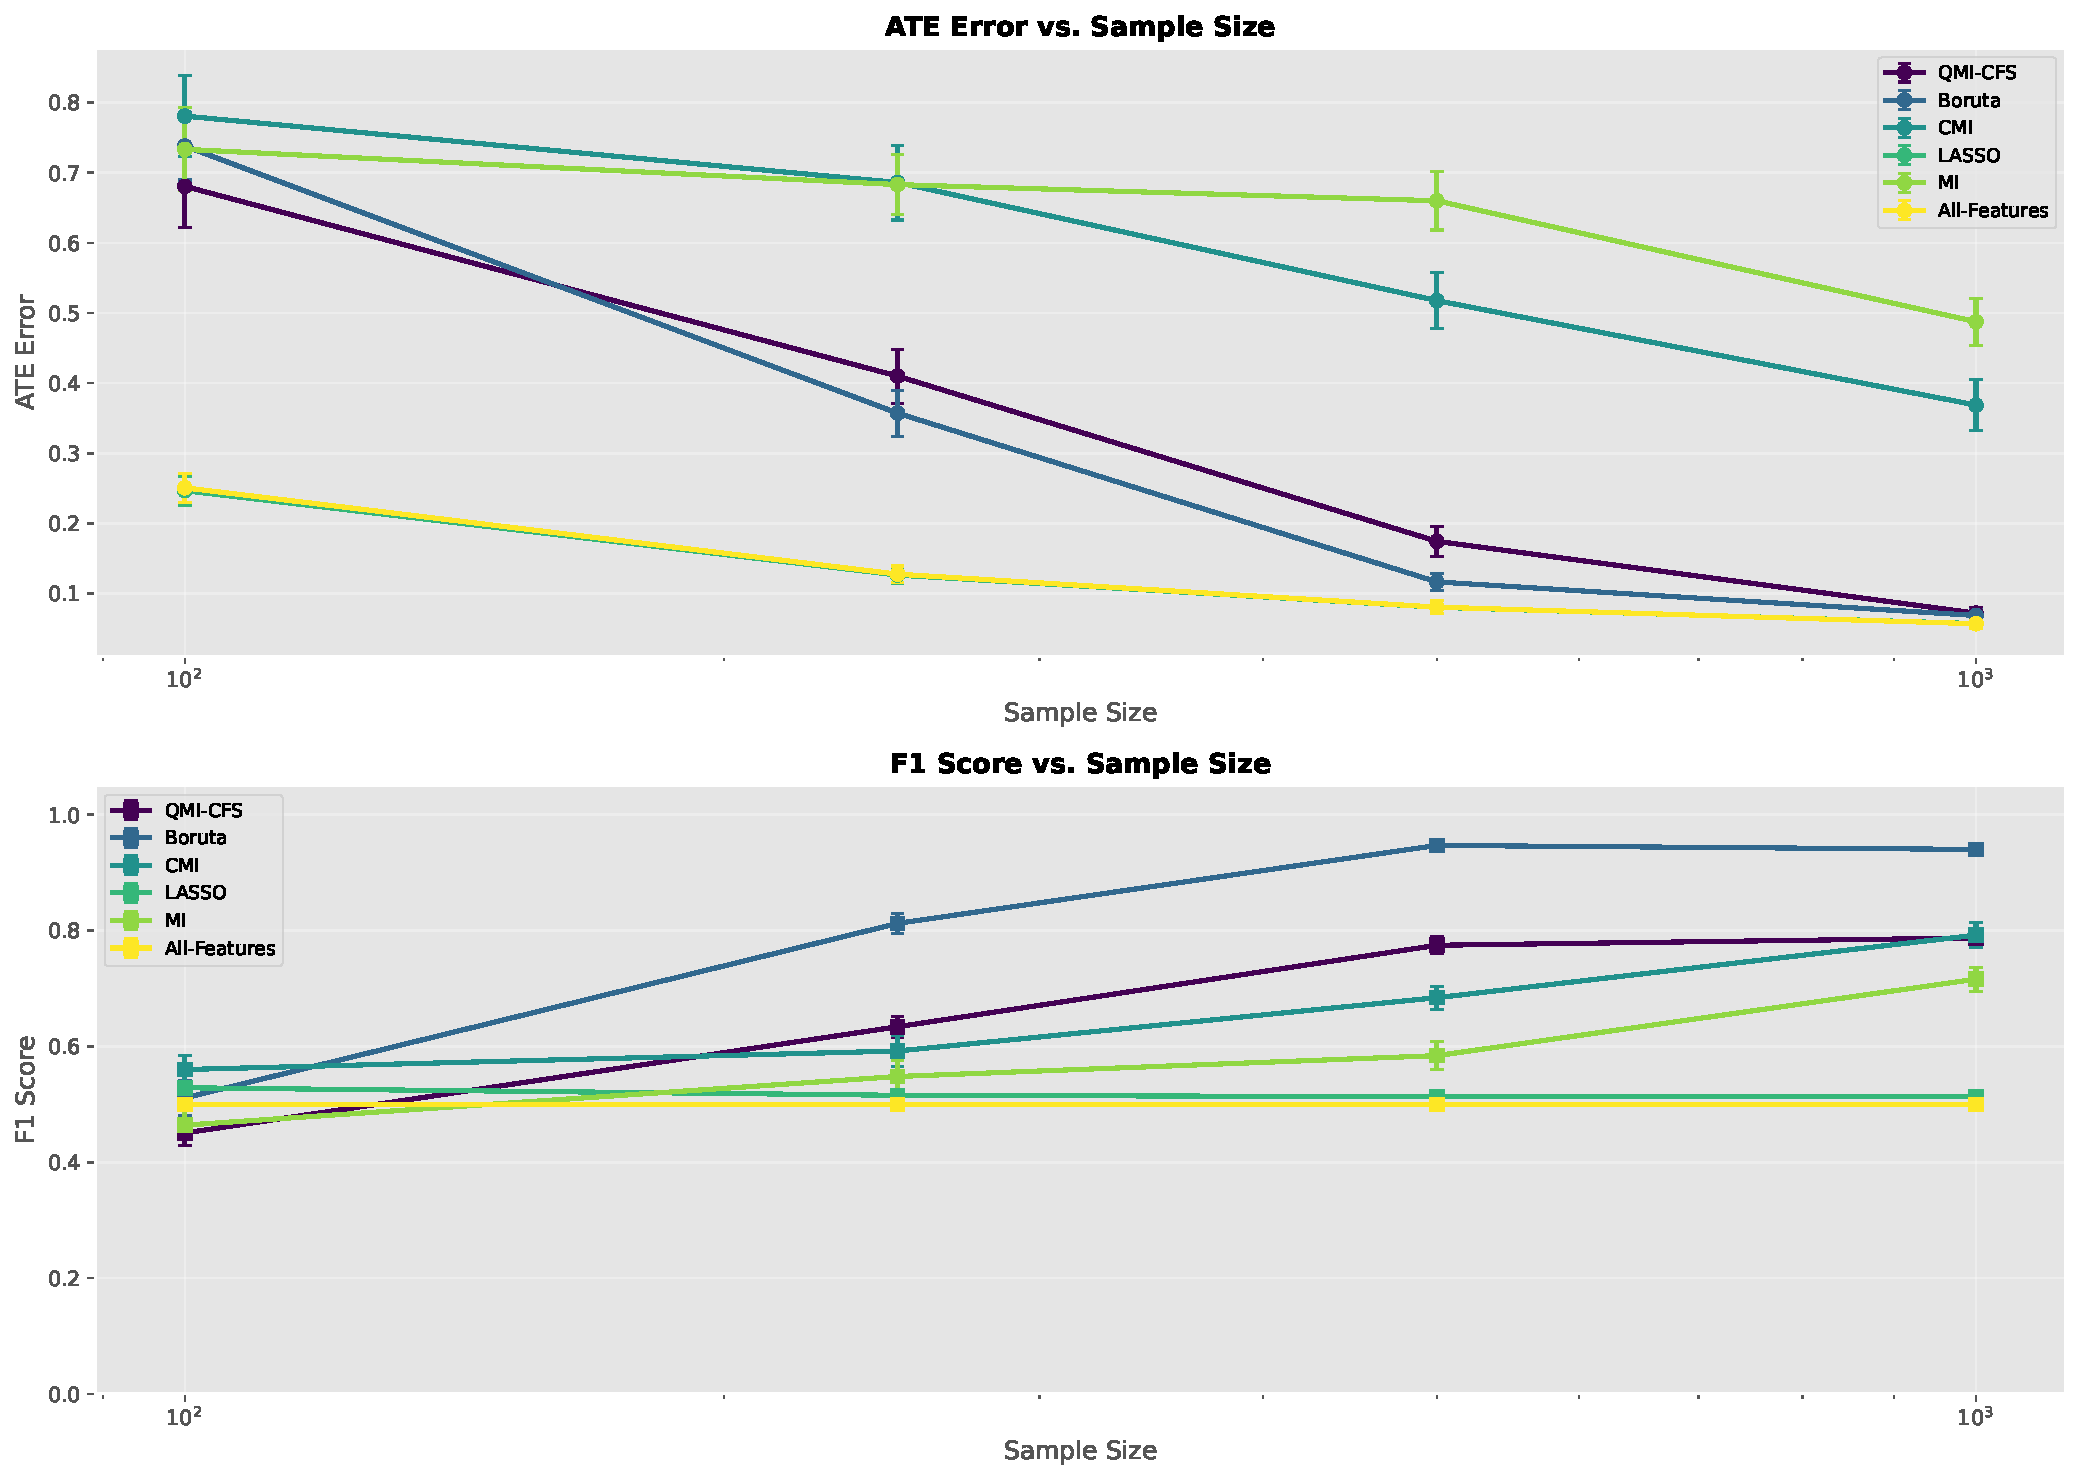
\includegraphics[width=\textwidth]{figures/v3_small_sample.pdf}
    \caption{Small-sample behavior: F1 score (left) and ATE error (right) vs. sample size on the LLD DGP. Error bars show standard error.}
    \label{fig:small_sample}
\end{figure}

\subsection{Ablation Study}
\label{sec:ablation}

Table~\ref{tab:ablation} examines QMI-CFS components. Removing bootstrap stability screening (``No Bootstrap'') generally degrades performance on cleaner datasets (LLD, HDS) because it selects too many features, but it can help on weak-signal datasets (WC, IC) where the lower variance of a single selection step is beneficial. Removing the pairwise term (``No Pairwise'') often produces similar or slightly better F1 than the full method, confirming that pairwise QMI is not a major driver of performance. The Conservative and Precision weight configurations trade precision for recall in a dataset-dependent manner.

\input{tables/table6_ablation.txt}

\subsection{Interaction Confounding: An Exploratory Sensitivity Analysis}
\label{sec:interacting}

The IC dataset is specifically designed so that no individual feature has a strong marginal effect: both treatment assignment and outcome depend on products $X_0X_1$, $X_2X_3$, and $X_4X_5$. Table~\ref{tab:f1} and Figure~\ref{fig:ic} show that CMI achieves the highest F1 ($0.425$). The pairwise-augmented QMI-CFS ($0.332$) is slightly worse than classic QMI-CFS ($0.339$) and only modestly better than MI ($0.345$), confirming that pairwise QMI provides little benefit.

\begin{figure}[htbp]
    \centering
    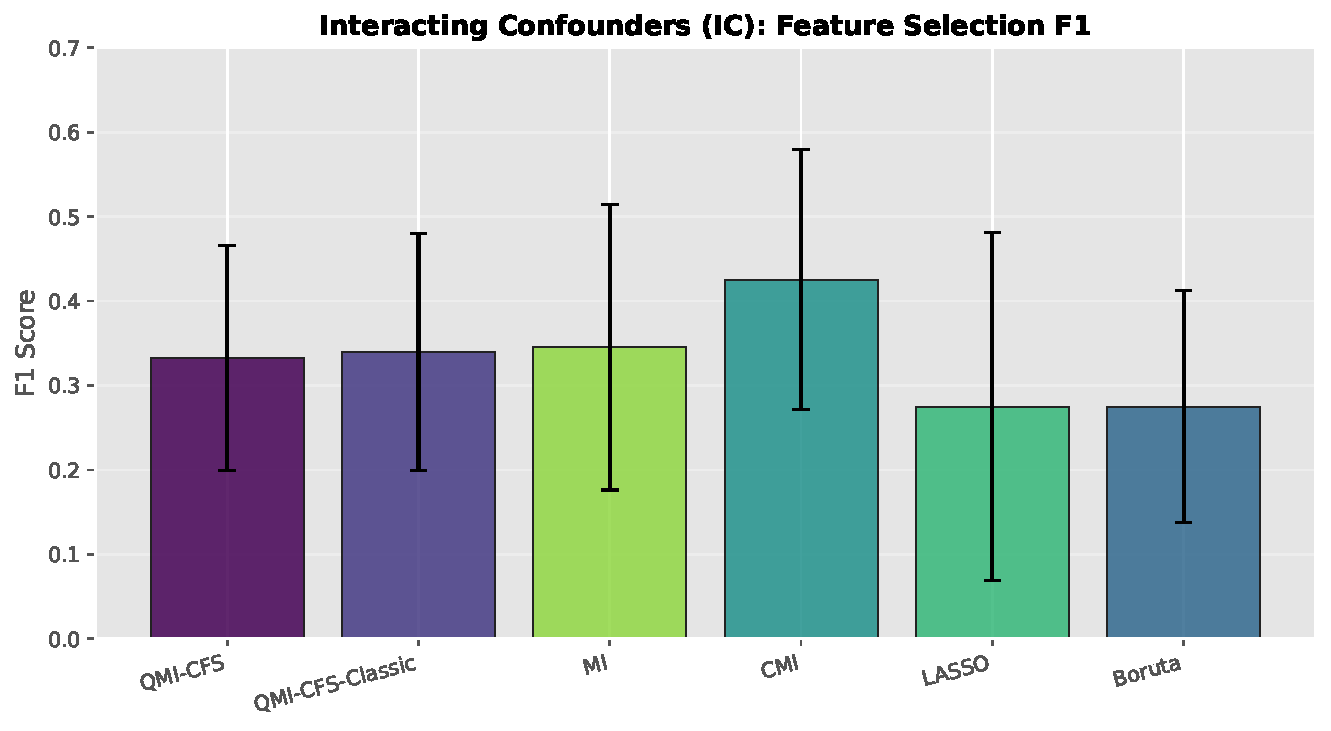
\includegraphics[width=0.75\textwidth]{figures/v3_ic_comparison.pdf}
    \caption{Interacting Confounders (IC) dataset: feature-selection F1. \textbf{QMI-CFS} uses the composite QMI score plus adaptive pairwise entanglement (neighbors=2); \textbf{QMI-CFS-Classic} is the same composite score without the pairwise term. CMI outperforms both QMI-CFS variants on this interaction-heavy DGP.}
    \label{fig:ic}
\end{figure}

Table~\ref{tab:ic_ate} reports ATE errors on IC. With linear AIPW, all methods fail. With a basic random-forest AIPW (an exploratory, lightly-tuned sensitivity analysis), QMI-CFS's ATE error improves only marginally ($2.027 \to 1.975$). This suggests that (a) the selected features do not fully capture the interacting structure, and (b) even flexible nuisance models struggle to learn the interactions from $n=500$ samples when only main-effect features are provided. These findings answer RQ3: dependency-based selectors face a fundamental limitation under interaction confounding.

\input{tables/table7_ic_ate.txt}

\section{Discussion}
\label{sec:discussion}

\textbf{When does QMI-CFS help?} QMI-CFS replaces k-NN density estimation with a deterministic density-matrix construction. This avoids the bandwidth/neighbor-count sensitivity of k-NN MI and provides a structured geometric objective. Relative to kernel-based dependence measures such as HSIC, QMI sidesteps kernel bandwidth selection and yields a bounded, parameter-free score once the encoding is fixed; a direct empirical comparison with HSIC is left for future work. Empirically, QMI-CFS improves over MI on most synthetic datasets for both feature recovery and ATE error, improves consistently with sample size, and achieves the best ATE error on IHDP. LASSO remains competitive on approximately linear DGPs.

\textbf{When do tree-based methods win?} Tree-based wrappers achieve higher F1 on several synthetic DGPs because they model interactions and thresholds directly. Their advantage is largest when confounders have strong, clean marginal or interaction signals. QMI-CFS does not claim to replace these methods; it offers a complementary, principled information-theoretic criterion.

\textbf{F1 vs. ATE divergence.} The IHDP result is the clearest example: QMI-CFS has lower F1 than CMI but yields the most accurate ATE estimate. This can occur when a method selects a subset that is well-calibrated for the nuisance models used downstream, even if it misses some true confounders or includes some instruments. It suggests that for causal inference, feature-selection evaluation should report both recovery metrics \textit{and} downstream causal estimation metrics.

\textbf{Limitations of extensions.} The pairwise QMI augmentation and the random-forest AIPW extension are best viewed as exploratory sensitivity analyses, not as core contributions. Pairwise QMI yields inconsistent and often negligible gains. The random-forest AIPW helps on genuinely nonlinear DGPs (NLC, WC) but overfits on linear or near-linear DGPs (LLD, HDS, CC) and barely helps on IC. These findings temper the expectation that quantum-inspired or lightly-tuned nonlinear extensions alone will solve interacting-confounder problems.

\paragraph{QMI vs.\ kernel-based dependency measures.} QMI-CFS is related to classical kernel methods because angle encoding defines a feature map $\phi(\mathbf{x})$ and the density matrix is built from outer products in that mapped space. However, QMI differs from HSIC in three ways. First, QMI uses von Neumann entropy on density matrices rather than an RKHS norm, so no kernel bandwidth must be selected at estimation time. Second, the trace-one density-matrix construction regularizes the dependency estimate. Third, the composite QMI score explicitly combines propensity, prognostic, and conditional terms, whereas HSIC measures undirected dependency. These differences are methodological; whether they translate into empirical advantages depends on the data-generating process, as our honest comparison shows.

\textbf{Broader limitations.} First, QMI-CFS assumes unconfoundedness (all confounders measured). Second, computational cost is $O(B \cdot n \cdot d)$ for single-feature scores; the optional pairwise augmentation adds $O(n \cdot d^2)$, and the constant is dominated by small eigenvalue decompositions. Third, angle encoding is a design choice; alternative encodings may behave differently. Fourth, all experiments are classical simulations; NISQ hardware implementation is future work. Fifth, we have not compared against BART, Causal Forest, or DragonNet.

\section{Conclusion}
\label{sec:conclusion}

This paper reframes QMI-CFS not as a universally superior algorithm but as a case study in quantum-information-inspired dependency measures for causal feature selection. We asked whether Quantum Mutual Information can identify confounders competitively with classical selectors (RQ1), whether better confounder recovery leads to better treatment-effect estimation (RQ2), and how dependency-based selectors behave under interaction confounding (RQ3).

Our empirical answers are modest but clear. QMI-CFS is competitive with classical information-theoretic methods on feature recovery and achieves the lowest ATE error on IHDP, but it is not dominant: tree-based wrappers outperform it on several synthetic DGPs, and all dependency-based selectors struggle when confounding is driven by feature interactions. Most importantly, confounder-recovery F1 and downstream ATE error are essentially uncorrelated across our benchmarks ($R^2 \approx 0.04$). The IHDP result exemplifies this divergence: QMI-CFS has lower F1 than CMI yet yields the most accurate causal estimate.

These findings suggest two practical lessons. First, quantum-inspired dependency measures are best understood as structured, parameter-free alternatives to classical kernel-based scores rather than sources of quantum advantage. Second, future evaluations of causal feature-selection methods should jointly report feature-recovery and downstream causal-estimation metrics, because the two need not align.

Future work includes: (i) direct empirical comparison with HSIC-based selectors (RBF-HSIC with median and cross-validated bandwidths, HSIC-Lasso) to test the parameter-free-kernel claim more directly, (ii) data-driven or cross-validated selection of the QMI weights $(\alpha,\beta,\gamma)$, (iii) inclusion of BART and Causal Forest baselines, (iv) stronger, computable finite-sample bounds on QMI estimation error, (v) more sophisticated nonlinear AIPW with cross-validated nuisance models, (vi) NISQ hardware implementation, and (vii) extensions to mediation analysis and instrumental variable settings.

%  - - Bibliography  - -
\begin{thebibliography}{99}

\bibitem{pearl2009causality}
Pearl, J.: Causality: Models, Reasoning, and Inference, 2nd edn. Cambridge University Press (2009)

\bibitem{imbens2015causal}
Imbens, G.W., Rubin, D.B.: Causal Inference for Statistics, Social, and Biomedical Sciences: An Introduction. Cambridge University Press (2015)

\bibitem{fleuret2004fast}
Fleuret, F.: Fast binary feature selection with conditional mutual information. Journal of Machine Learning Research \textbf{5}, 1531-1555 (2004)

\bibitem{tsamardinos2003algorithms}
Tsamardinos, I., Aliferis, C.F., Statnikov, A.: Algorithms for large scale Markov blanket discovery. In: FLAIRS Conference. pp. 376-381 (2003)

\bibitem{tibshirani1996regression}
Tibshirani, R.: Regression shrinkage and selection via the lasso. Journal of the Royal Statistical Society: Series B (Methodological) \textbf{58}(1), 267-288 (1996)

\bibitem{belloni2014inference}
Belloni, A., Chernozhukov, V., Hansen, C.: Inference on treatment effects after selection among high-dimensional controls. Review of Economic Studies \textbf{81}(2), 608-650 (2014)

\bibitem{kursa2010boruta}
Kursa, M.B., Rudnicki, W.R.: Feature selection with the Boruta package. Journal of Statistical Software \textbf{36}(11), 1-13 (2010)

\bibitem{breiman2001random}
Breiman, L.: Random forests. Machine Learning \textbf{45}(1), 5-32 (2001)

\bibitem{kraskov2004estimating}
Kraskov, A., St\"{o}gbauer, H., Grassberger, P.: Estimating mutual information. Physical Review E \textbf{69}(6), 066138 (2004)

\bibitem{koller1996toward}
Koller, D., Sahami, M.: Toward optimal feature selection. In: International Conference on Machine Learning. pp. 284-292 (1996)

\bibitem{yu2020causality}
Yu, K., Guo, X., Liu, L., Li, J., Wang, H., Ling, Z., Wu, X.: Causality-based feature selection: Methods and evaluations. ACM Computing Surveys \textbf{53}(5), 1-36 (2020)

\bibitem{nielsen2010quantum}
Nielsen, M.A., Chuang, I.L.: Quantum Computation and Quantum Information: 10th Anniversary Edition. Cambridge University Press (2010)

\bibitem{havlivcek2019supervised}
Havl\'{i}\v{c}ek, V., C\'{o}rcoles, A.D., Temme, K., Harrow, A.W., Kandala, A., Chow, J.M., Gambetta, J.M.: Supervised learning with quantum-enhanced feature spaces. Nature \textbf{567}(7747), 209-212 (2019)

\bibitem{schuld2021supervised}
Schuld, M.: Supervised quantum machine learning models are kernel methods. arXiv:2101.11020 [quant-ph] (2021)

\bibitem{vedral2002role}
Vedral, V.: The role of relative entropy in quantum information theory. Reviews of Modern Physics \textbf{74}(1), 197-234 (2002)

\bibitem{kiriakidou2024mutual}
Kiriakidou, N., Diou, C.: Mutual information-based neighbor selection method for causal effect estimation. Neural Computing and Applications \textbf{36}(9), 4759-4773 (2024)

\bibitem{schreiber2000measuring}
Schreiber, T.: Measuring information transfer. Physical Review Letters \textbf{85}(2), 461-464 (2000)

\bibitem{gao2021efficient}
Gao, M., Aragam, B.: Efficient Bayesian network structure learning via local Markov boundary search. arXiv:2110.06082 [stat.ML] (2021)

\bibitem{curth2021inductive}
Curth, A., van der Schaar, M.: On inductive biases for heterogeneous treatment effect estimation. In: Advances in Neural Information Processing Systems. vol. 34, pp. 15,883-15,895 (2021)

\bibitem{curth2021really}
Curth, A., Svensson, D., Weatherall, J., van der Schaar, M.: Really doing great at estimating CATE? A critical look at ML benchmarking practices in treatment effect estimation. In: NeurIPS Datasets and Benchmarks Track (2021)

\bibitem{mucke2023feature}
M\"{u}cke, S., Heese, R., M\"{u}lle, S., Wolter, M., Piatkowski, N.: Feature selection on quantum computers. Quantum Machine Intelligence \textbf{5}(1), 11 (2023)

\bibitem{mummaneni2024miqubo}
Pranji\'{c}, D., Mummaneni, B.C., Tutschku, C.: Quantum annealing based feature selection in machine learning. arXiv:2411.19609 [cs.LG] (2024)

\bibitem{flores2026quantum}
Flores-Garrig\'{o}s, G., Albino Simen, A., et al.: Quantum feature selection with higher-order binary optimization on trapped-ion hardware. arXiv:2604.26834 [quant-ph] (2026)

\bibitem{vergara2017qmifs}
Vergara, J.R., Est\'{e}vez, P.A.: A review on feature selection methods based on mutual information. Neurocomputing \textbf{30}, 168-175 (2014)

\bibitem{hill2011bayesian}
Hill, J.L.: Bayesian nonparametric modeling for causal inference. Journal of Computational and Graphical Statistics \textbf{20}(1), 217-240 (2011)

\bibitem{wager2018estimation}
Wager, S., Athey, S.: Estimation and inference of heterogeneous treatment effects using random forests. Journal of the American Statistical Association \textbf{113}(523), 1228-1242 (2018)

\bibitem{shi2019adapting}
Shi, C., Blei, D., Veitch, V.: Adapting neural networks for the estimation of treatment effects. In: Advances in Neural Information Processing Systems. vol. 32 (2019)

\bibitem{gretton2005measuring}
Gretton, A., Bousquet, O., Smola, A., Sch\"{o}lkopf, B.: Measuring statistical dependence with Hilbert-Schmidt norms. In: Algorithmic Learning Theory. pp. 63-77 (2005)

\bibitem{gretton2007kernel}
Gretton, A., Fukumizu, K., Teo, C.H., Song, L., Sch\"{o}lkopf, B., Smola, A.J.: A kernel statistical test of independence. In: Advances in Neural Information Processing Systems. vol. 20, pp. 585-592 (2007)

\bibitem{gretton2012kernel}
Gretton, A., Borgwardt, K.M., Rasch, M.J., Sch\"{o}lkopf, B., Smola, A.: A kernel two-sample test. Journal of Machine Learning Research \textbf{13}(1), 723-773 (2012)

\bibitem{vansteelandt2012model}
Vansteelandt, S., Bekaert, M., Claeskens, G.: On model selection and model misspecification in causal inference. Statistical Methods in Medical Research \textbf{21}(1), 7-30 (2012)

\end{thebibliography}

\end{document}
